\documentclass{uebblatt}

\usepackage{draftwatermark}
\definecolor{pink}{rgb}{0.95,0.9,0.95}
\SetWatermarkText{\textsf{\textcolor{pink}{ENTWURF}}}
\SetWatermarkScale{1}

\newcommand{\Ch}{\mathrm{Ch}}

\begin{document}

\maketitle{13}{}

\begin{aufgabe}{Lokale Präsentierbarkeit der Kategorie der Kettenkomplexe}
Zeige, dass die Kategorie~$\Ch_{\geq0}(R)$ über einem Ring~$R$ lokal
präsentierbar ist.
\end{aufgabe}

\begin{aufgabe}{Die Dold--Kan-Korrespondenz}
\begin{enumerate}
\item Sei~$V_\bullet \in \Ch_{\geq0}(R)$. Konstruiere einen
simplizialen~$R$-Modul~$\Gamma(V)$ mit~$\Gamma(V_\bullet)_m = \bigoplus_{[m]
\twoheadrightarrow [k]} V_k$ (direkte Summe über alle monotonen
Surjektionen~$[m] \to [k]$).
\item Sei~$X$ ein simplizialer~$R$-Modul. Sei~$CX_\bullet$ der Kettenkomplex
mit~$(CX)_m = X_m$ und Differential~$d = \sum_i (-1)^i X(\partial^i)$.
Sei~$DX_\bullet$ der Unterkomplex der degenerierten Ketten. Sei~$NX_\bullet =
CX_\bullet/DX_\bullet$. Was ist~$N(\Delta[n])$?
\item Zeige, dass die Kategorie der simplizialen~$R$-Moduln vermöge~$\Gamma$
und~$N$ zur Kategorie der Kettenkomplexe von~$R$-Moduln (in nichtnegativen
Graden) äquivalent ist.
\item Wie ist auf der Kategorie der simplizialen~$R$-Moduln eine
Modellstruktur zu definieren, damit diese Quillen-äquivalent
zu~$\Ch_{\geq0}(R)$ wird?
\end{enumerate}
\end{aufgabe}

\begin{aufgabe}{Ringwechsel}
Sei~$R \to S$ ein Ringhomomorphismus. Zeige, dass
Skalarerweiterung und -einschränkung eine Quillen-Adjunktion bezüglich der
projektiven Modellstrukturen bilden.
\[ \left(\begin{array}{@{}rcl@{}}
  \Ch_{\geq0}(R) &\longrightarrow& \Ch_{\geq0}(S) \\
  V_\bullet &\longmapsto& V_\bullet \otimes_R S
\end{array}\right)\ \text{\huge$\dashv$}\ \left(\begin{array}{@{}rcl@{}}
  \Ch_{\geq0}(S) &\longrightarrow& \Ch_{\geq0}(R) \\
  W_\bullet &\longmapsto& W_\bullet
\end{array}\right) \]
\vspace{-1em}
\end{aufgabe}

\begin{aufgabe}{Die Ableitung des Tensorprodukts}
Sei~$k$ ein Körper. Seien~$f$ und~$g$ reguläre Elemente von~$k[x,y]$.
Berechne das abgeleitete Tensorprodukt~$k[x,y]/(f) \otimes_{k[x,y]}^\LL
k[x,y]/(g)$. Kannst du das Ergebnis geometrisch deuten?
\end{aufgabe}

\vfill
\centering
\href{https://en.wikipedia.org/wiki/Simplicial_homology}{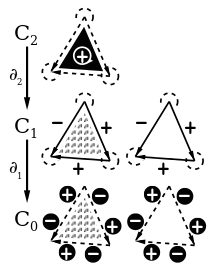
\includegraphics[scale=0.4]{images/simplicial-homology}}
\par

\end{document}

1) Dold-Kan zwischen simplizialen R-Moduln und Ch_*(R). Transport der
Modellstruktur auf sMod(R). Beweis, daß sMod(R) simpliziale kombinatorische
Modellkategorie ist.

4) Berechnung des Homotopietypes von Map(X, Y) in einem interessanten
Beispiel

5) Diskussion anderer Modellstrukturen auf Ch_*(R)?
